%%
%% Capítulo 2: Regras gerais de estilo
%%

\mychapter{Fundamentação científico-tecnológica}
\label{Cap:fundamentacao}

\section{Contextualização e problema}
\label{contextualização}

% Falar um pouco sobre o cenário mundial de eólica

% Falar sobre o problema com desempenho das máquinas

% Falar das tecnologias utilizadas

% Falar da robustez do sistema

% Falar do valor agregado

O setor energético é o principal insumo dos mais variados setores da economia, sendo item fundamental para o desenvolvimento econômico e social. Para que este setor consiga acompanhar e alavancar os avanços da sociedade, devemos investir cada vez mais em desenvolvimento de novas tecnologias, bem como aumentar o acesso da sociedade às fontes mais eficientes e limpas de energia.

A energia eólica é vista como uma das mais promissoras fontes de energia, pela sua crescente utilização e investimentos, tendo apresentado nos últimos anos uma evolução exponencial da capacidade eólica instalada. Atualmente os países lideres em geração de energia eólica são, China, Estados Unidos da América e Alemanha. Em 2010 a China tornou-se o país com a maior capacidade instalada no mundo, sendo atualmente responsável por 35\% do total da capacidade instalada, seguida pelos Estados Unidos, que possuem 17\% do total \cite{global-wind-energy}. Na figura \ref{Fig:ranking-mundial-capacidade-instalada} é demonstrado o ranking mundia de capacidade instalada, no qual o Brasil ocupa a 8ª posição.

\begin{figure}[htbp!] \begin{center}
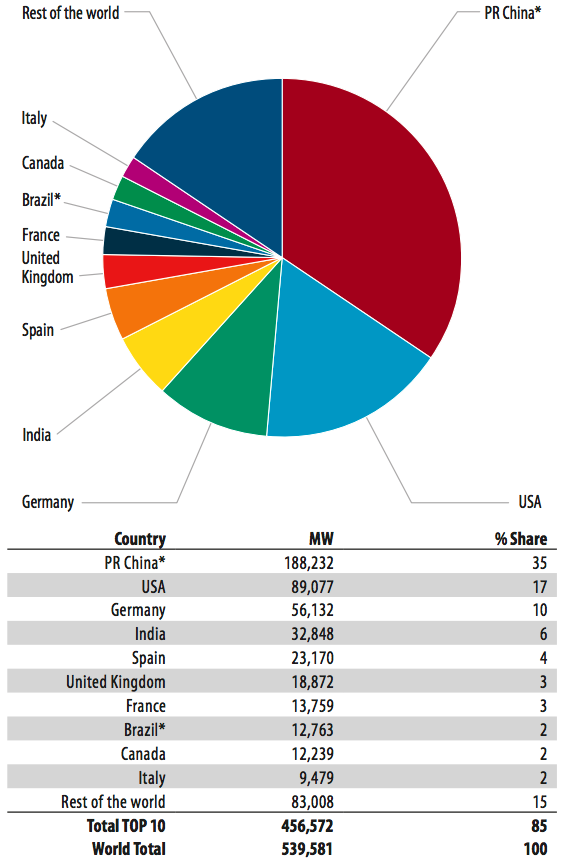
\includegraphics[width=0.75\linewidth]{./figuras/grafico-capacidade-instalada-mundo}
\caption{Ranking mundia de capacidade instalada}
\label{Fig:ranking-mundial-capacidade-instalada}
\end{center} 
\end{figure}

O Brasil recebe destaque no cenário mundial pelo elevado potencial eólico e pelo volume de geração de energia por fonte eólica, que tem crescido consideravelmente nos últimos anos. Com 508 usinas no total, o ano de 2017 terminou com 12,77 GW de potência eólica instalada, o que representou um crescimento de 18,87\% de potência em relação a dezembro de 2016, quando a capacidade instalada era de 10,74 GW \cite{boletim-anual-geracao-2017}.

Em 2017 foram instalados no país 6,84 GW de potência, considerando todas as fontes de geração de energia elétrica. Desse crescimento, 47,86\% corresponde a fonte hidroelétrica e 29,62\% a fonte eólica. Com esse acréscimo de 2,03 GW de capacidade instalada, o total eólico permitiu para a fonte uma participação de 8,10\% da matriz elétrica brasileira, como pode ser observado no gráfico \ref{Fig:matriz-energetica-brasileira}, que apresenta a participação de todas as fontes de geração na matriz elétrica brasileira no final de 2017 \cite{boletim-anual-geracao-2017}.

\begin{figure}[htbp!] \begin{center}
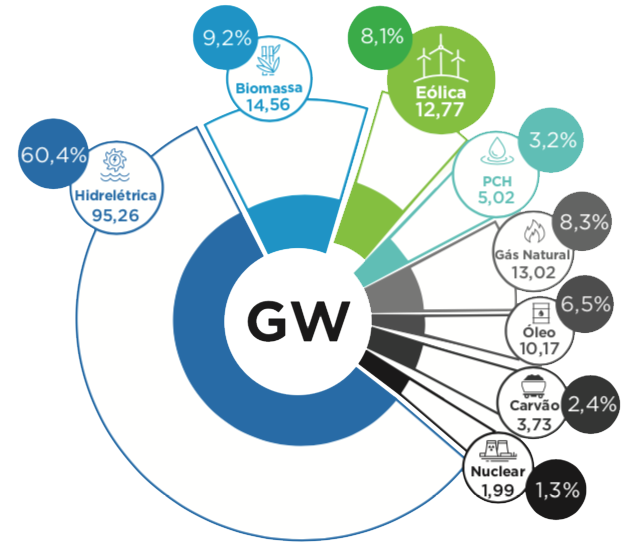
\includegraphics[width=0.65\linewidth]{./figuras/matriz-energetica-brasileira}
\caption{Matriz energética brasileira}
\label{Fig:matriz-energetica-brasileira}
\end{center} 
\end{figure}

Sendo um dos países que mais investe em energia eólica no mundo, o Brasil também é considerado um dos mais atrativos para investimentos em energias renováveis. A fonte eólica, sozinha, foi responsável por cerca de 80\% dos investimentos em renováveis no país de 2005 até 2015 \cite{CENARIO}. Um dos maiores motivos do alto investimento em energia eólica no Brasil é o alto valor do fator de capacidade proporcionado pelos ventos brasileiros. O fator de capacidade aponta o aproveitamento do vento para produção de energia e é representado pela proporção entre a geração efetiva da usina em um intervalo de tempo e a sua potência instalada. Em 2017 o valor médio do fator de capacidade no Brasil foi de 42,9\%, tendo atingido maior fator mensal médio em setembro, com 60,6\%, enquanto que no restante do mundo a média do é de 24,7\%\cite{boletim-anual-geracao-2017}.

O crescimento da utilização da força dos ventos para a produção de energia atribui-se principalmente ao desenvolvimento tecnológico no setor, que elevou a competitividade em relação ao preço, quando comparado com outras fontes geradoras de energia elétrica. Entretanto, a implantação de parques eólicos ainda exige um alto nível de investimento inicial \cite{matrizes-energeticas-brasil}. Esse fato justifica o incentivo à realização de pesquisa e a busca de inovações nesta área.

O contributo social desta pesquisa é fornecer uma ferramenta que irá possibilitar o aumento da eficiência dos parques, conferindo, consequentemente, maior competitividade para a fonte eólica frente às demais fontes de geração, o que pode estimular a modicidade tarifária, a qual preconiza o consumo de energia mais barata para o cidadão brasileiro. Além disso, incentivar a expansão de fontes renováveis de energia, que não agridem o meio ambiente, é contribuir para o bem-estar humano.

% Focar mais no problema

\subsection{Conceitos preliminares}
\label{Sec:conceitosPreliminares}

\subsubsection{O aerogerador}
\label{Sec:oAerogerador}

Aerogeradores basicamente são dispositivos projetados para transformar energia cinética dos ventos em algum tipo de energia mecânica. Os aerogeradores podem ser classificados de acordo com a orientação de seu rotor entre aerogerador de eixo vertical ou de eixo horizontal.

A maioria dos aerogeradores modernos utilizados comercialmente possuem em sua maioria eixo horizontal, três pás e um sistema de transmissão baseado em caixa multiplicadora. A figura \ref{Fig:ilustracaoAerogerador} ilustra os principais componentes de um aerogerador. São eles:

\begin{itemize}
    \item \textbf{Rotor:} Localizado no topo da torre, é composto pelo conjunto do hub e das pás. É o responsável por transferir a energia do vento através do torque para o eixo principal.
    \item \textbf{Nacele:} Compartimento instalado no alto da torre que armazena os elementos responsáveis pala conversão da energia mecânica em energia elétrica.
    \item \textbf{Torre:} Elemento que sustenta o rotor e a nacele na altura apropriada ao seu funcionamento.
    \item \textbf{Yaw:} Sistema responsável pela rotação da nacele (controle de giro), especialmente para o posicionamento do rotor de forma perpendicular à direção do vento.
    \item \textbf{Sistema de transmissão:} Composto pelo eixo principal e a caixa multiplicadora. O eixo principal transmite o torque gerado a partir da rotação das pás em uma frequência baixa. A caixa multiplicadora é responsável por elevar esta frequência de rotação até a entrada do gerador. Existem modelos de aerogeradores denominados de \textit{direct drive}, o torque do rotor é levado diretamente ao gerador, eliminando a necessidade de uso de caixa multiplicadora.
    \item \textbf{Sistema Elétrico:} Composto por toda a parte de conversão, transmissão de energia e controle do aerogerador. O principal subcomponente deste sistema é o gerador.
\end{itemize}

\begin{figure}[htbp!] \begin{center}
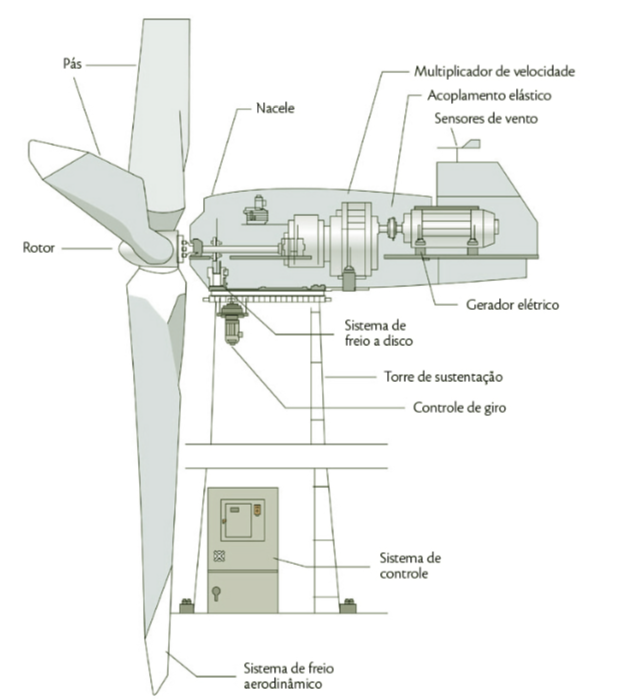
\includegraphics[width=0.75\linewidth]{./figuras/ilustracao-aerogerador}
\caption{Componentes de um aerogerador}
\label{Fig:ilustracaoAerogerador}
\legend{Fonte: \cite{componentes-aerogerador}}
\end{center} 
\end{figure}

\subsubsection{Sistema SCADA}
\label{Sec:scada}

Os Sistemas SCADA (Supervisory Control and Data Aquisition), ou sistemas supervisórios, são sistemas comumente utilizados na automação industrial que utilizam computação e comunicação para automatizar o monitoramento e controlar processos industriais. Eles permitem que os dados de um determinado processo produtivo sejam monitorados e rastreados. Esses dados são coletadas continuamente através de sensores e posteriormente, enviados para o computador central que faz o gerenciamento dos dados.

Os sistemas supervisórios são essenciais para o funcionamento de um parque eólico. Através deles os operadores conseguem controlar e armazenar os dados dos aerogeradores, torres anemométricas e subestações. Dentre os dados armazenados pelo sistema SCADA são encontrados informações da potência, da velocidade do vento na nacele, a orientação da nacele, temperaturas, pressões, entre outros. A partir desses dados contidos no SCADA é possível identificar falhas, calcular a quantidade de energia gerada, ter acesso a disponibilidade dos aerogeradores, etc.


\subsubsection{Curva e coeficiente de potência}
\label{Sec:curvaDePotencia}

A potência de uma turbina eólica varia de acordo com a velocidade do vento e cada turbina tem uma curva característica de desempenho de energia. Com essa curva é possível prever a produção de energia de um aerogerador, sem considerar detalhes técnicos de seus componentes. Assim, a curva de potência é um gráfico que indica qual a potência elétrica disponível no aerogerador para diferentes velocidades de vento \cite{iec-power-performance}.

A quantidade de potência disponível no vento que pode ser convertida em potência mecânica por um aerogerador, é chamado de coeficiente de potência ($c_p$). Esse coeficiente indica é utilizado para comparar a eficiência entre diferentes aerogeradores. Na figura \ref{Fig:ilustracaoCurvaPotencia} é demonstrado o gráfico com a curva e o coeficiente de potência de um aerogerador. 

\begin{figure}[htbp!] \begin{center}
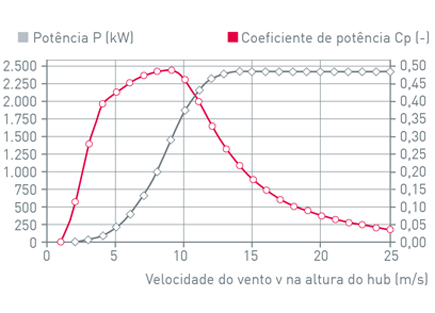
\includegraphics[width=0.75\linewidth]{./figuras/curva-potencia-wobben}
\caption{Curva de potência de um aerogerador}
\label{Fig:ilustracaoCurvaPotencia}
\legend{Fonte: \cite{catalogo-wobben-e92}}
\end{center} 
\end{figure}

\section{Desempenho de aerogeradores}
\label{Sec:desempenhoDeAerogeradores}

O risco de um investimento em um parque eólico esta fortemente atrelado as diferenças entre a produção efetiva e a produção estimada durante a elaboração do projeto. A partir disso surge a necessidade do acompanhamento do funcionamento dos parques eólicos para que seja garantido o bom desempenho dos aerogeradores.

A metodologia aplicada para o acompanhamento do desempenho dos parques, na maioria das vezes está prevista no contrato entre a empresa dona do parque eólico e a empresa fabricante dos aerogeradores e nesse caso essa verificação assume também um caráter de garantia no qual eventuais desvios podem originar penalizações, caso o desempenho seja abaixo do contratual.

A grande maioria dos contratos entre os fabricantes e os parques eólicos levam em consideração a disponibilidade dos aerogeradores como parâmetro para acompanhamento do desempenho. Esse indicador não é efetivo para medir o desempenho e sim apenas uma contabilização do tempo em que as máquinas estiveram em operação ou em condições de operação.

O desempenho de um aerogerador depende essencialmente da sua curva de potência e da sua disponibilidade. 

\subsubsection{Curva de potência}
\label{Sec:curvaPotenciaDesempenhoAerogeradores}

Como mencionado anteriormente, a curva de potência de um aerogerador é uma curva característica que expressa a potência gerada em função da velocidade do vento. Essa ferramenta é essencial para avaliação de desempenho de um aerogerador, tanto para previsão de produção, como para avaliação dos resultados obtidos. Entretanto, a curva de potência garantida pelo fabricante de aerogerador e a curva obtida com a turbina em funcionamento nem sempre são iguais. Além do local onde é feita a garantia da curva de potência e do local onde opera o aerogerador serem diferentes, existem outras razões pelas quais podem existir desvios no comportamento da curva de potência. Algumas razões são:

\begin{itemize}
  \item \textbf{Turbulência:} Pode ser definida como alterações na média da velocidade do vento em curtos períodos de tempo (ordem de segundos ou menos). Normalmente é gerada por conta da fricção com a superfície, causado pela topografia, e efeitos térmicos, por conta da variação da temperatura.
  \item \textbf{Efeito esteira:} Uma vez que a turbina eólica produz energia mecânica a partir da energia do vento incidente, o vento que "sai" da turbina tem um conteúdo energético muito menor que o do vento que "entrou". Pode ser definida como alterações na média da velocidade do vento que passou pelo rotor, podendo diminuir até um terço da velocidade inicial, formando uma esteira de vento turbulento. O diâmetro da esteira aumenta conforme o vento se afasta do rotor e se dissolve com uma distância média de 10 diâmetros do rotor.
  \item \textbf{Operação com limitação de potência:} Toda as turbinas são desenvolvidas com algum sistema de controle de potência. Para evitar danos ao equipamento é necessário limitar a potência mecânica do aerogerador durante ventos com velocidade acima da velocidade nominal de operação. Caso essa limitação de potência ocorrer por um longo período de tempo, trará prejuízos consideráveis ao parque eólico.
  \item \textbf{Deterioração e danificação nas pás:} A função das pás é converter, através da força de sustentação, a energia cinética do vento em energia mecânica. O seu desenho é feito para converter o máximo de energia possível, logo, o desgaste desta ao longo do tempo claramente afeta o desempenho aerodinâmico, afetando a sustentação gerada e consequentemente a potência retirada.
  \item \textbf{Condições climáticas:} Condições climáticas imprevistas podem afetar o desempenho de um aerogerador. Um exemplo são as baixas temperaturas, onde o gelo formado nas pás podem alterar o desempenho aerodinâmico, levando a perda energética. Outros casos que podem afetar o desempenho são a presença de insetos ou poeira, nas pás da turbina.
\end{itemize}

\subsubsection{Disponibilidade}
\label{Sec:disponibilidadeDesempenhoAerogeradores}



\section{Histórico}
\label{Sec:historico}
% * Surgimento da LogAp
% * Falar sobre o know how em desenvolvimento de software para indústria
% * Surgimento do projeto Windbox

Não há um número mínimo ou máximo de páginas para propostas de tema,
dissertações ou teses. Entretanto, se o seu documento for muito menor
do que a média pode transmitir uma ideia de falta de conteúdo a
apresentar. Por outro lado, um documento muito grande corre o risco de
só conseguir a atenção total do leitor no seu início, fazendo com que
as partes mais importantes, que geralmente estão no final do
documento, não sejam devidamente consideradas. Apenas para servir como
parâmetro, estão indicados a seguir os limites usuais quanto ao número
de páginas\footnote{Uma folha corresponde a uma página em impressão em
face simples e a duas páginas em impressão em face dupla} dos
documentos do PPgEEC da UFRN, adotando as margens e os espaçamentos
definidos neste modelo:
\begin{itemize}
\item Proposta de tema para exame de qualificação de mestrado:
entre 20 e 40 páginas
\item Proposta de tema para exame de qualificação de doutorado:
entre 30 e 50 páginas
\item Dissertação de mestrado:
entre 50 e 100 páginas
\item Tese de doutorado:
entre 80 e 150 páginas
\end{itemize}

O tamanho padrão para a fonte é de 12pt.  Para facilitar a escrita de
comentários, sugestões e correções da banca, recomenda-se o espaçamento
1.5 entre as linhas do texto e a impressão em um único lado da folhas
para os seguintes documentos:
\begin{itemize}
\item Proposta de tema para exame de qualificação;
\item Versão inicial de dissertação de mestrado; e
\item Versão inicial de tese de doutorado.
\end{itemize}
Para as versões finais de teses e dissertações, onde se busca uma
melhor qualidade visual e tipográfica do texto, deve-se utilizar
espaçamento simples entre as linhas e a impressão nos dois lados da
página.

As margens devem seguir os valores adotados neste documento, que podem
ser verificados no arquivo \texttt{principal.tex}. É importante notar
que, na versão final de teses ou dissertações, recomenda-se a
impressão nos dois lados da página. Por esta razão, a margem direita
em páginas pares deve ter o mesmo valor que a margem esquerda em
páginas impares e vice-versa, para que a encadernação fique
correta. Também em razão da impressão em frente e verso, os capítulos
devem sempre começar em uma página de número ímpar, com a eventual
inclusão de uma página em branco. O \LaTeX\ se encarrega de fazer
automaticamente estes ajustes.

\section{Robustez do sistema}
\label{RobustezSistema}

Documentos do porte de uma tese ou dissertação devem ser subdivididos
em capítulos. O capítulo deve conter uma introdução e um fecho.

A introdução do capítulo fornece ao leitor uma breve descrição do que
será tratado no capítulo e não forma uma seção: para exemplificar, a
introdução deste capítulo é o parágrafo que precede a primeira seção.

O fecho do capítulo apresenta comentários finais sobre o que foi
desenvolvido no capítulo e/ou faz uma ligação com o que será visto no
capítulo seguinte; normalmente é colo cado em uma seção específica,
denominada ``Comentários Finais'', ``Conclusões'', ``Resultados'',
``Avaliação Final'' ou qualquer outra denominação que se adéque ao
texto.

Capítulos são divididos em seções. O número ideal de seções é
impossível de se precisar. Entretanto, um capítulo com uma única seção
provavelmente deve ser agregado ao capítulo anterior ou posterior. Um
capítulo com quinze seções provavelmente deve ser subdividido em dois
capítulos.

Capítulos, seções e subseções devem ser rotulados para que possam ser
referenciados em qualquer parte do texto.  Isto é feito com o comando
\verb|\label{}|, que deve ser colocado logo após (nunca antes) o
comando que criou a seção, capítulo, etc. O parâmetro do comando
\texttt{label} é o nome simbólico que será usado para se fazer
referência a esta entidade dentro do texto, com o comando
\verb|\ref{}|. O nome pode ser qualquer coisa, mas não pode conter
acentos, por exemplo. Neste documento nós utilizamos a convenção de
prefixar os rótulos dos capítulos com \texttt{Cap:}, das seções com
\texttt{Sec:}, das equações com \texttt{Eq:} e assim por diante, mas
esta convenção não é obrigatória. Veja a seguir um exemplo de
utilização das referências cruzadas:
% quotation é um ambiente para citações, que ficam "recuadas" em
% relação ao resto do texto
\begin{quotation}
\dots no capítulo~\ref{Cap:Introducao} apresentamos um modelo de
capítulo de tese.
\end{quotation}
Note que, no código fonte deste trecho de frase, o espaço entre a palavra
\texttt{capítulo} e o comando \verb|\ref{}| foi escrito com
um \texttt{\~{}} e não com um espaço normal. O \texttt{\~{}} é o
comando \LaTeX\ para criar um espaço onde não se pode mudar de linha,
pois ficaria estranho se o texto ``no capítulo'' estivesse no fim de
uma linha e o número \ref{Cap:Introducao} no início da outra linha.

Existe uma particularidade no código fonte do parágrafo anterior. Para
se escrever:
\begin{quotation}
\dots o comando \LaTeX\ para criar\dots
\end{quotation}
se colocou depois do comando \verb|\LaTeX| um espaço
precedido de uma contrabarra, ao invés de um espaço normal. Isto porque
espaços depois de comandos são ignorados pelo \LaTeX; com um espaço
% Na linha anterior não houve necessidade do espaço com contrabarra
% depois do comando \LaTeX, pois ele é seguido por um ; e não um espaço
normal as palavras ficariam ligadas:
\begin{quotation}
\dots o comando \LaTeX para criar\dots
\end{quotation}
Ao invés do espaço precedido pela contrabarra, poder-se-ia também
utilizar um \texttt{\~{}}. A diferença é que neste caso o \LaTeX\ não
poderia fazer uma quebra de linha entre as palavras.
